\documentclass{beamer}
\usetheme{Warsaw}

\usepackage{blkarray}
\usepackage{bigstrut}
\usepackage{amsmath}
\usepackage{bbm}

\makeatletter
\let\BA@quicktrue\BA@quickfalse
\makeatother

\title{Higher Order Markov Chains and Spacey Walks}
\author{Nicolas Nytko}
\date{\today}

\begin{document}
\frame{\titlepage}

% Overview
\begin{frame}
  \frametitle{Overview}
  \begin{enumerate}
  \item Introduction/review of first-order Markov chains
  \item Higher order Markov chains, relation to tensors
  \item Stochastic walks on higher order Markov chains
  \item Applications of the Spacey walk
  \end{enumerate}
\end{frame}


% Review of first-order markov chains
\begin{frame}
\frametitle{Markov Chains}
{\bf Markov Chains} are stochastic models describing a sequence of states with a probability of transitioning between each.
\begin{itemize}
\item Defined as matrix: ${\bf P} \in \mathbb{R}^{n\times n}$, ${\bf P}_{ij}$ gives probability of moving to state $i$ from $j$, for chain with $n$ states.
\item Given distribution/state vector ${\bf x}^{(n)}$, one step of a random walk is represented by matrix-vector product ${\bf x}^{(n+1)} = {\bf P} {\bf x}^{(n)} \enskip \Leftrightarrow \enskip x^{(n+1)}_i = \sum_j P_{ij} x^{(n)}_j $.
\end{itemize}

\begin{block}{}
\begin{columns}
\begin{column}{0.5\linewidth}
\centering
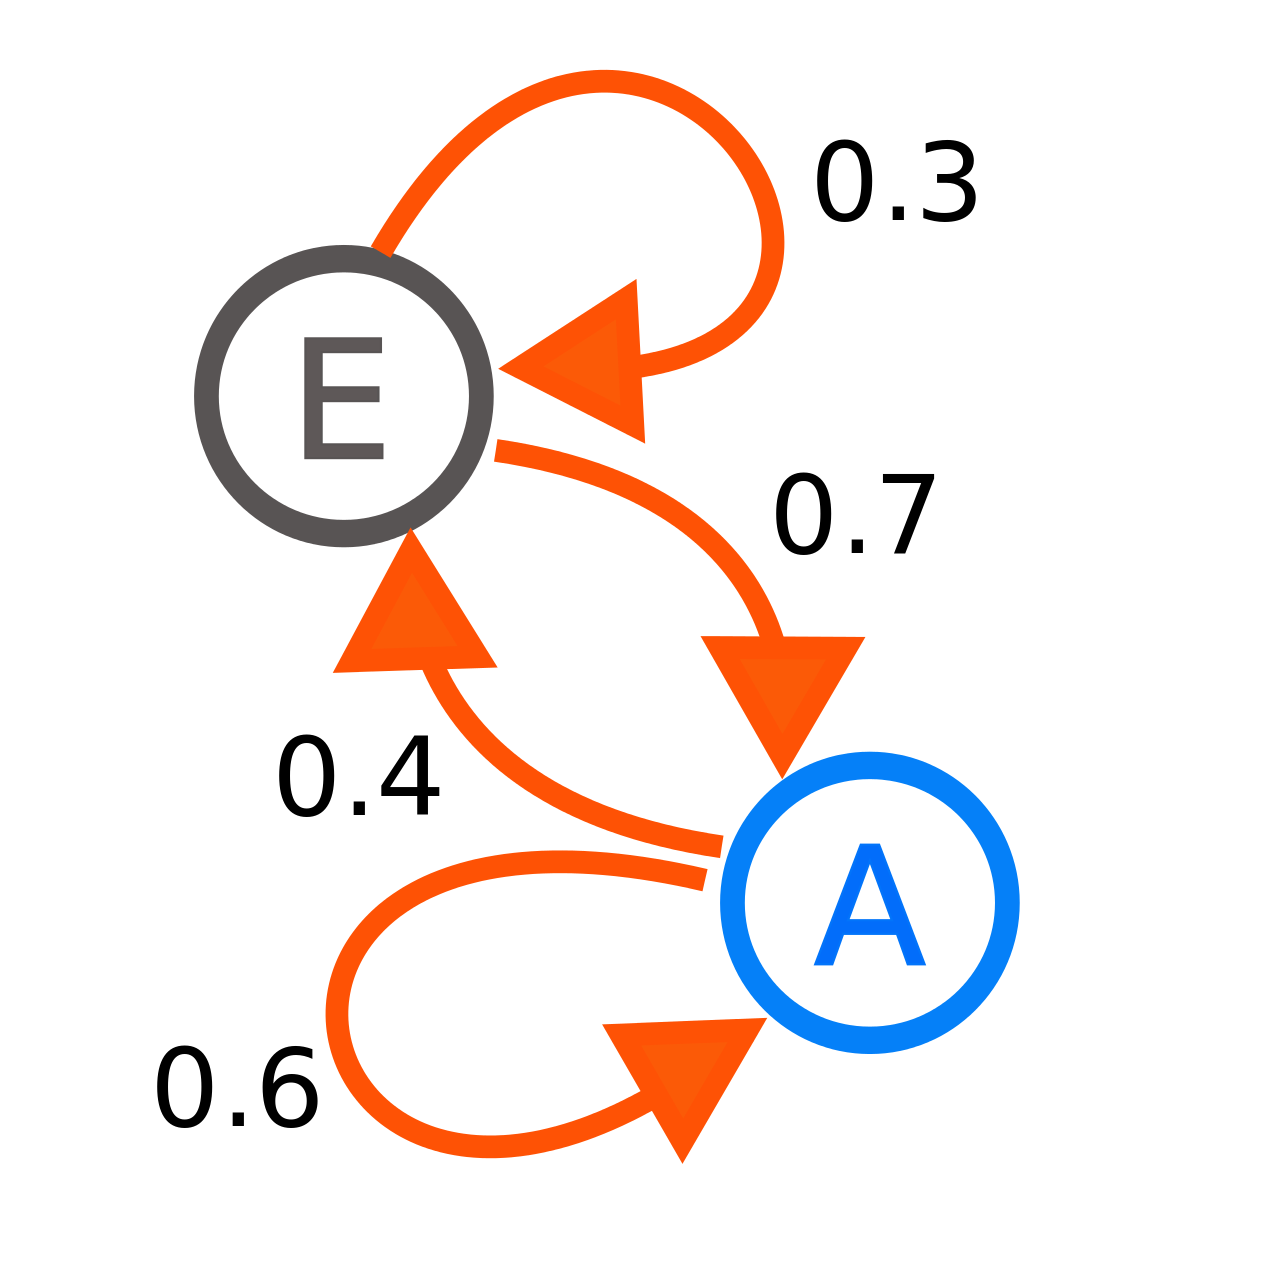
\includegraphics[scale=0.072]{images/markov.png}
\end{column}

\begin{column}{0.5\linewidth}
\centering
Transition matrix:
\[{\bf P} =
\begin{blockarray}{ccc}
  & A & E \\
	\begin{block}{c[cc]}
		\bigstrut[t]
		A & 0.6 & 0.7 \\
		E & 0.4 & 0.3
		\bigstrut[b] \\
	\end{block}
\end{blockarray}
\]
\end{column}
\end{columns}

\begin{center}
\begin{tiny}
Figure from \url{https://commons.wikimedia.org/wiki/File:Markovkate_01.svg}
\end{tiny}
\end{center}
\end{block}

\end{frame}


% Various definitions
\begin{frame}
\frametitle{Definitions}
\begin{block}{Time Homogeneous}
Each transition probability is independent of the time step $t$.
\end{block}

\begin{block}{Irreducible}
Every state can be reached from every other state.
\end{block}

\begin{block}{Periodic}
Periodic markov chain:
\[ \exists i \in S \quad s.t. \quad \left(P^d\right)_{ii} \neq 0; \quad d\in\mathbb{Z},d>1 \]
Periodicity implies a state may only return to itself after some multiple $d$ ``hops''.  If every state has self loops the chain is \textbf{aperiodic}.
\end{block}

\end{frame}


% Examples
\begin{frame}
\frametitle{Canonical Examples}

\textbf{Google PageRank}
\begin{itemize}
\item Markov chain represents the ``idealized'' web surfer.  States are webpages and transition probability is given by number of outgoing links between pages.
\item Ranking is determined by probability of being on certain page.
\end{itemize}

\textbf{Board Games}
\begin{itemize}
\item Each spot on game board is a state.
\item Probability of moving between spots is given by dice, spinner, etc.
\end{itemize}

\textbf{Weather}
\begin{itemize}
\item States are possible weather conditions.
\item Tomorrow's weather is randomly chosen based on today's conditions.
\end{itemize}

\end{frame}


% Introduction of steady-state distribution
\begin{frame}
\frametitle{Steady-State Distribution}

\begin{block}{}
\textbf{Steady state} vector $\boldsymbol{\pi} \in \mathbb{R}^n$ does not change when multiplied by Markov chain:
\[ \boldsymbol{\pi} = {\bf P} \boldsymbol{\pi} \]
\end{block}

\begin{itemize}
\item Average distribution as random walk tends to length infinity, $\lim_{k\to\infty} {\bf P}^k{\bf x}$
\item Is equivalent to \textbf{Perron vector} of matrix, dominant eigenvector with nonnegative components.
\item Compute iteratively with power method: ${\bf x}^{(k+1) } = {\bf Px}^{(k)}$.
\end{itemize}

\begin{block}{}
Unique steady states are guaranteed for \textbf{irreducible}, \textbf{aperiodic} Markov chains.
\end{block}

\end{frame}

% Introduce higher order chains as matricised tensors
\begin{frame}
\frametitle{Markov Chains with Memory}
What if we want our chain to \textbf{remember} where it has been?  Introduce $\boldsymbol{m}$-\textbf{order Markov chain}, where transition probability depends on previous $m$ states.

\begin{itemize}
\item Probability is now stored as ${\bf P} \in \mathbb{R}^{n \times n^m}$, where columns are a $m$-tuple of each state permutation.
\item Random step becomes slightly more complicated than just a \textit{mat-vec}, will see a better way of doing this.
\end{itemize}

\begin{block}{}

\[
{\bf P} =
\begin{blockarray}{ccccc}
& \left(s_0, s_0\right) & \left(s_1 , s_0\right) & \left(s_0, s_1\right) & \left(s_1, s_1\right) \\
 \begin{block}{c[cccc]}
	\bigstrut[t]
	s_0 & p_{1,1} & p_{1,2} & p_{1,3} & p_{1,4} \\
	s_1 & p_{2,1} & p_{2,2} & p_{2,3} & p_{2,4}
	\bigstrut[b] \\
 \end{block}
\end{blockarray}
\]

\centering
\begin{tiny}
(Example indexing for $2^{\text{nd}}$ order chain with $n=2$ states.)
\end{tiny}

\end{block}

\end{frame}

% Introduce higher order chain
\begin{frame}
\frametitle{Higher Order Markov Chains}

We can \textbf{fold the last dimension} of the higher-order Markov matrix to obtain a higher dimensional \textbf{tensor}.

\begin{block}{}
Order $m$ Markov chain with $n$ states is order $m+1$ tensor

\[\mathcal{P} \in \mathbb{R}^{\overbrace{n\times n\times \cdots \times n}^{m+1\text{ dimensions}}}\]

Transition probability indexed by $P_{i_{(n+1)},i_{(n)},i_{(n-1)},\ldots,i_{(n-m+1)}}$
\end{block}

\begin{itemize}
\item State/distribution is stored as order $m$ tensor.
\item Example random step for order 2 Markov chain: $X^{(n+1)}_{ij} = \sum_k P_{ijk} X^{(n+1)}_{jk}$
\end{itemize}

\end{frame}

% Notation
\begin{frame}
\frametitle{Tensor Notation}
\begin{itemize}

\item Will write tensors as flattening along first mode, i.e. for $\mathcal{P} \in \mathbb{R}^{2 \times 2 \times 2}$:
	\[ \mathcal{P} = \left[
      \begin{array}{@{}cc|cc@{}}
        p_{111} & p_{121} & p_{112} & p_{122} \\
        P_{211} & p_{221} & p_{212} & p_{222}
      \end{array}
    \right]
 \]	
\item Each slice is referred to as a \textbf{panel}, enumerates transition probabilities given some previous state.
 
\item Note each panel is its own \textbf{stochastic matrix}.
\end{itemize}
\end{frame}

% Higher order markov as tensor
\begin{frame}
\frametitle{Higher Order Steady-State Distribution}

Assume 2nd order chains in following slides for notational simplicity -- everything generalizes to higher orders though.

\begin{block}{}
\textbf{Steady state} tensor ${\bf X} \in \mathbb{R}^{n \times n}$ does not change when multiplied along first mode.
\[ X_{ij} = \sum_k P_{ijk} X_{jk} \]
\end{block}
\begin{itemize}
\item Conceptually simple, but requires $\mathcal{O}\left(n^m\right)$ space to store state tensor.
\end{itemize}
\begin{block}{}
Replace state tensor with \textbf{low rank approximation} ${\bf x} \in \mathbb{R}^n$:
\[ x_i = \sum_{jk} P_{ijk} x_j x_k \]
Actually just the \textbf{$\boldsymbol{z}$-eigenvector} of $\mathcal{P}$!
\end{block}

\end{frame}

% Stochastic process
\begin{frame}
\frametitle{Stochastic Processes}

\begin{itemize}
\item For first order, steady state/eigenvector can be represented by a {\bf random walk}.
\item Our low rank transformation:
\[ X_{ij} = \sum_k P_{ijk} X_{jk} \quad \Rightarrow \quad x_i = \sum_{jk} P_{ijk} x_j x_k \]
is algebraic, is there a {\bf stochastic} process?
\end{itemize}

\end{frame}


% Spacey walks
\begin{frame}
\frametitle{Spacey Walks}

Present the concept of a \textbf{spacey walk}: upon reaching a new state we \textit{space out} and forget all previous states.  State history is then \textbf{randomly made up} from previously seen states.

\begin{block}{}

Let $X\left(0\right), X\left(1\right), \ldots, X\left(n\right)$ be the sequence of visited states and $N$ to be the number of states.  Define $Y\left(n\right)$ as a random previously seen state, each weighted by number of occurrences:

\begin{equation*}
P\left(Y(n) = k \:|\: \mathcal{F}_n \right) = \frac{1}{n+N}\left(1 + \sum_{s=1}^n \mathbbm{1}\left(X\left(s) = k\right) \right) \right)
\end{equation*}

Transition probability is then given by:

\begin{equation*}
P\left(X\left(n+1\right) = i \:|\: X(n) = j, Y(n) = k\right) = P_{ijk}
\end{equation*}

\end{block}

\end{frame}


% Polya Urn
\begin{frame}
  \frametitle{P\'{o}lya Urn}
  \begin{columns}
    \begin{column}{0.4\linewidth}
      \centering
      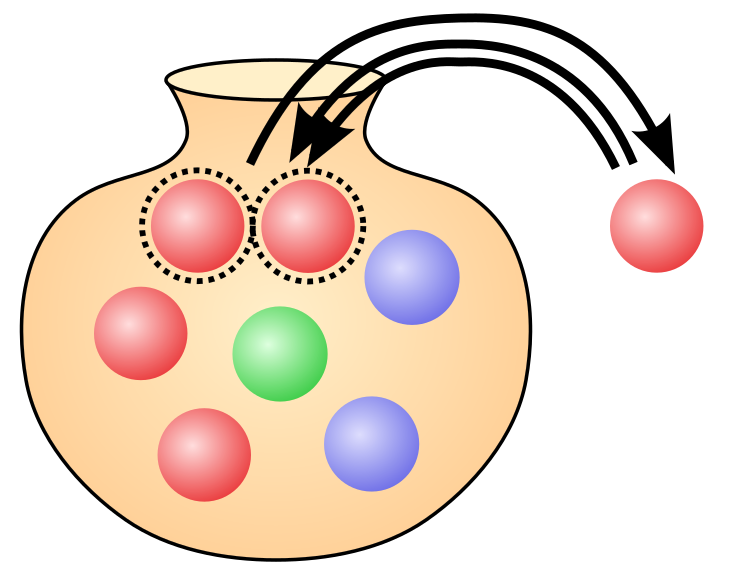
\includegraphics[width=\linewidth]{images/polya.png}
      \begin{center}
		\tiny
		\url{https://commons.wikimedia.org/wiki/File:Urn_problem_qtl5.svg}
      \end{center}
    \end{column}
    \begin{column}{0.6\linewidth}
      For simple example of the Spacey walk, consider \textbf{P\'{o}lya Urn} process.  Have urn with red and green balls inside, and repeat the following process:
      \begin{enumerate}
      \item Select a random ball from the urn
      \item Put the random ball back in the urn
      \item Put another ball of same selected color in the urn
      \end{enumerate}

      \[ \mathcal{P}_{\left(1\right)} =
        \left[
          \begin{array}{@{}cc|cc@{}}
            1 & 1 & 0 & 0 \\
            0 & 0 & 1 & 1
          \end{array}
        \right]
      \]
    \end{column}
  \end{columns}
\end{frame}


% Vertex-reinforced random walk
\begin{frame}
  \frametitle{Vertex-reinforced random walks}
  This spacey walk is an instance of a \textbf{vertex-reinforced random walk}.  I.e., a walk that always picks next state based on transition probabilities, but probabilities evolve over time.

  \begin{block}{Vertex-reinforced walk}
    \begin{equation*}
      w_i\left(n\right) = \frac{1}{N+n}\left(1 + \sum_{s=1}^n \mathbbm{1}\left(X(s)=i\right) \right)
    \end{equation*}
    \begin{equation*}
      P\left(X(n+1) = i \:|\: \mathcal{F}_n\right) = \left[{\bf M} \left({\bf w}(n)\right)\right]_{i,X\left(n\right)}
    \end{equation*}

    Where ${\bf M}$ maps the \textit{occupation vector} ${\bf w}$ to a stochastic matrix ${\bf P}\in\mathbb{R}^{N\times N}$.
  \end{block}

  For spacey walks, define:
  \[ M\left({\bf w}\right) = \sum_{k=1}^N P_{:,:,k} w_k \]
\end{frame}


% Vertex walk <=> ODE
\begin{frame}
  \frametitle{Vertex-reinforced walks and ODEs}
  Why care about turning the \textbf{spacey walk} into a \textbf{vertex-reinforced walk}?
  \begin{block}{}
    Lets us model chain as a \textbf{dynamical system}:
    \[ \frac{d{\bf x}}{dt} = \pi\left({\bf M}\left({\bf x}\right)\right) - {\bf x} \]
    For some $\pi$ that maps transition matrices to a stationary distribution.
  \end{block}
  So, to find the tensor eigenvector ${\bf x}$, we can solve the ODE for its \textbf{fixed points}:
  \[ \frac{d{\bf x}}{dt} = 0 \quad \Longleftrightarrow \quad x_i = \sum_{ij}P_{ijk}x_jx_k \]
\end{frame}


% ODE <=> Tensor Z-Eigenvector
\begin{frame}
  \frametitle{Solution to Steady State}
  \begin{itemize}
  \item Now reduced eigenvector problem to matter of \textbf{integrating an ODE}.
  \item Can offer better convergence properties than traditional power method/fixed point iteration.
  \item Take following periodic Markov chain as example:
  \end{itemize}
  \[ \mathcal{F}_{\left(1\right)} =
    \left[
      \begin{array}{@{}cc|cc@{}}
        0 & 1 & 1 & 1 \\
        1 & 0 & 0 & 0
      \end{array}
    \right]
  \]

  \begin{columns}
    \begin{column}{0.5\linewidth}
      When using power iteration:
      \[ {\bf x}^{n+1}_i = \sum_{jk} P_{ijk}x_jx_K \]
      Oscillates between $\begin{bmatrix}0&1\end{bmatrix}^T$ and $\begin{bmatrix}1&0\end{bmatrix}^T$.
    \end{column}
    \begin{column}{0.5\linewidth}
      Forward-stepping ODE
      \[ \frac{d{\bf x}}{dt} = \pi\left({\bf M}\left({\bf x}\right)\right) - {\bf x} \]
      with Euler converges to analytical solution $\begin{bmatrix} \left(\sqrt{2}-1\right)/2 & \left(3-\sqrt{5}\right)/2  \end{bmatrix}^T$.
    \end{column}
  \end{columns}
\end{frame}

% Population Genetics
\begin{frame}
  \frametitle{Population Genetics}
  \textbf{Population genetics} study dynamics of allele distribution, or type of each organism.  Suppose we have $n$ types, the possibility of passing each type to child is given by:
  \[ P\left(\text{child is type } i \:|\: \text{parents are types } j, k\right) = P_{ijk} \]
  \begin{itemize}
  	\item Parent ordering doesn't matter, have natural symmetry $P_{ijk}=P_{ikj}$.
  	\item Spacey walk models how population dynamics evolve over time.
  	\item Stationary type distribution satisfies ${\bf x}_i = \sum_{jk}P_{ijk}x_jx_k$.
  \end{itemize}

\end{frame}

% Taxicab model
\begin{frame}
	\frametitle{Taxi Trajectory Modeling}
	\begin{columns}
		\begin{column}{0.3\linewidth}
			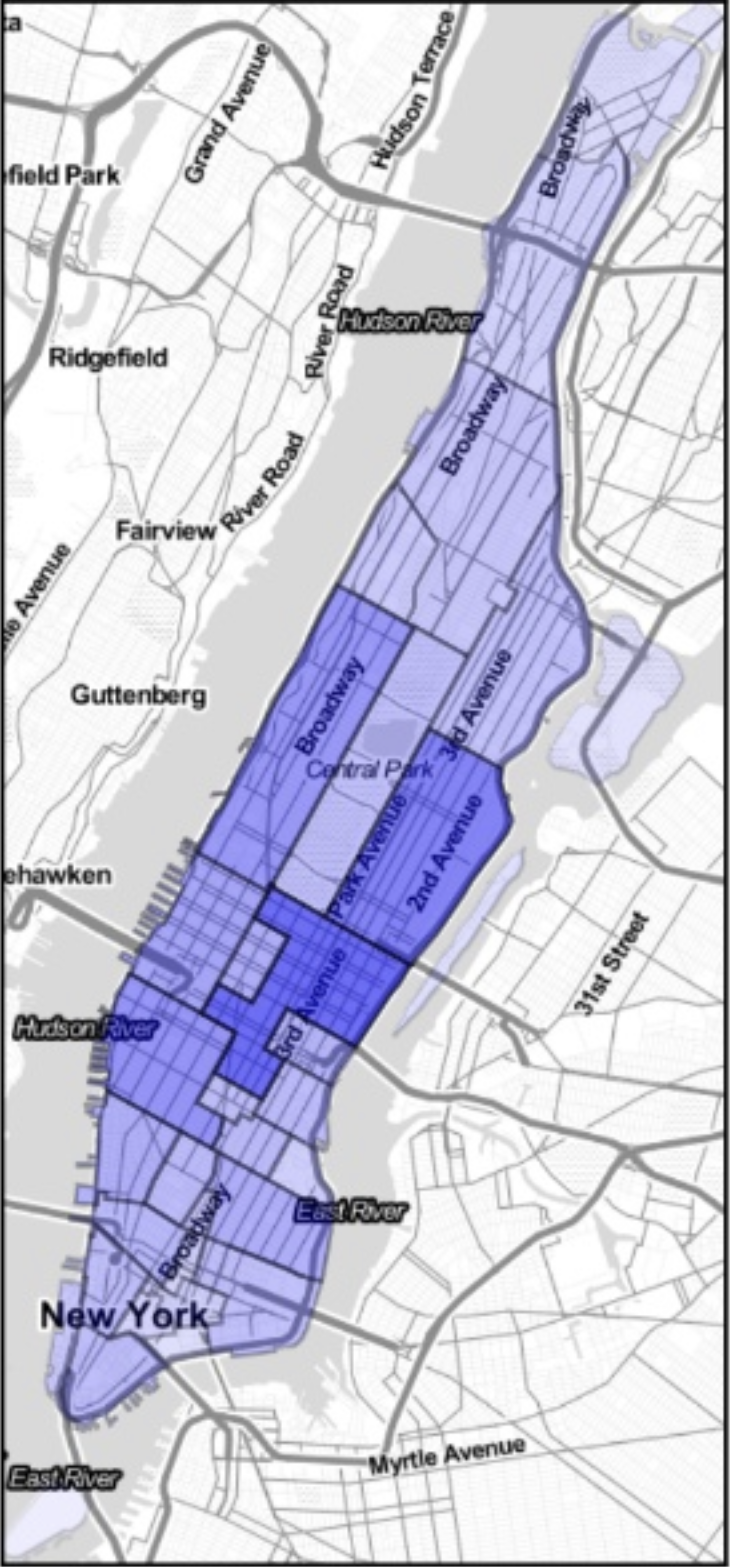
\includegraphics[width=\linewidth]{images/nytaxi.png}
			\begin{tiny}
				\begin{center}
					(Benson, Gleich, Lim)
				\end{center}
			\end{tiny}
		\end{column}

		\begin{column}{0.7\linewidth}
		\begin{itemize}
			\item Model taxicab as \textbf{spacey walk} $\mathcal{P}_{ijk}$, with $N$ states being possible locations.
			\item Passenger at location $k$ gets picked up at $j$ and goes to $i$ with probability $P_{ijk}$.
			\item Assume passengers are likely to be picked up nearby where they are dropped off, i.e. at airport.
			\item Difficult to solve, higher order gives better performance (RMSE) than first order:
		\end{itemize}
		\begin{tabular}{|ccc|}
			\hline
			First Order & Second Order & Spacey Walk \\
			\hline
			0.846 & 0.835 & 0.835 \\
			\hline
		\end{tabular}
		\end{column}
	\end{columns}
\end{frame}

% Conclusion
\begin{frame}
	\frametitle{Conclusion}
	\begin{itemize}
		\item Introduce high order Markov chain as having \textbf{memory of previous states}.
		\item High order Markov chains can be represented as \textbf{tensor} of transition probabilities.
		\item Tensor form naturally emits eigenvector steady-state.
		\item Z-eigenvector is the limiting distribution of the \textbf{spacey random walk}.
		\item Random walk can be turned into equivalent ODE construction.
		\item We can solve an ODE to find the tensor eigenvector!
		\item The Spacey walk is a generalization of the \textbf{P\'{o}lya process}, has interesting applications.
	\end{itemize}
\end{frame}


% References
\begin{frame}
\frametitle{References}
\nocite*{}
\bibliographystyle{plain}
\bibliography{ho-markov}
\end{frame}

\end{document}
